\documentclass{article}
\PassOptionsToPackage{numbers, compress}{natbib}
\usepackage[preprint]{neurips_2026}

% --- standard packages ---
\usepackage[utf8]{inputenc}
\usepackage[T1]{fontenc}
\usepackage[colorlinks=true,linkcolor=blue!70!black,citecolor=blue!70!black,urlcolor=blue!70!black]{hyperref}
\usepackage{url}
\usepackage{booktabs}
\usepackage{amsfonts}
\usepackage{nicefrac}
\usepackage{microtype}
\usepackage{xcolor}
\usepackage{graphicx}
\usepackage{subcaption}
\usepackage{amsmath}
\usepackage{amssymb}
\usepackage{amsthm}
\usepackage{algorithm}
\usepackage{algorithmic}
\usepackage{bm}
\usepackage{multirow}

% --- figure/table placement ---
\setcounter{topnumber}{1}
\setcounter{bottomnumber}{1}
\renewcommand{\topfraction}{0.5}

% --- theorem environments ---
\newtheorem{theorem}{Theorem}
\newtheorem{lemma}[theorem]{Lemma}
\newtheorem{proposition}[theorem]{Proposition}
\newtheorem{corollary}[theorem]{Corollary}
\theoremstyle{definition}
\newtheorem{definition}[theorem]{Definition}
\theoremstyle{remark}
\newtheorem{remark}[theorem]{Remark}

% --- custom commands ---
\newcommand{\R}{\mathbb{R}}
\newcommand{\E}{\mathbb{E}}
\newcommand{\Var}{\operatorname{Var}}
\newcommand{\Cov}{\operatorname{Cov}}
\newcommand{\sign}{\operatorname{sign}}
\newcommand{\eps}{\varepsilon}
\newcommand{\teps}{\tilde{\varepsilon}}
\newcommand{\gen}{\mathrm{gen}}
\newcommand{\real}{\mathrm{real}}
\newcommand{\eff}{\mathrm{eff}}

\title{Variance-Corrected Single-Index Composition for Heavy-Tailed Return Generators}

\author{%
  Jeffrey D.~Varner \\
  Robert Frederick Smith School of Chemical and Biomolecular Engineering\\
  Cornell University, Ithaca, NY 14850 \\
  \texttt{jdv27@cornell.edu} \\
}

\begin{document}

\maketitle

\begin{abstract}
% abstract.tex

Per-asset generators for synthetic financial returns, such as the
hidden Markov models with explicit jump components used in the
\texttt{JumpHMM.jl} package, are built to preserve marginal structure
(heavy tails, regime switching) but say nothing about cross-sectional
factor dependence. The standard fix is to compose each generator draw
with a single-index market factor, but the naive recipe inflates the
marginal variance by a term that grows quadratically in the factor
loading, distorting the very marginal the generator was designed to
preserve; replacing the generator residual with a Gaussian draw
eliminates the distortion but discards the marginal entirely. We
derived a closed-form variance correction that sits between these two
failure modes, rescaling the idiosyncratic draw by a scalar chosen so
that the composed series inherits the generator's marginal variance
exactly while recovering the calibrated factor loading. The correction
was paired with a sign-preserving clip that engaged whenever the market
component would have exceeded the generator variance, keeping defensive
assets defensive, and a separate branch for index-tracking assets
targeted the calibrated coefficient of determination rather than the
marginal, with the SPY-on-itself identity recovered as a degenerate
limit without special-casing. Branch selection was driven entirely by
the calibrated coefficient of determination, requiring no external
metadata, and each asset carried a persisted construction flag so
downstream consumers could audit which path it took. Evaluated on a $424$-ticker US equity and exchange-traded fund (ETF)
universe against the SPY market path with \texttt{JumpHMM.jl}
marginals, the hybrid construction recovered the factor loading to a
median absolute error of $0.018$ and passed a per-ticker
Kolmogorov--Smirnov test against the real marginal at rate $50\%$,
versus $4\%$ for the naive composition and below $1\%$ for the
Gaussian-residual baseline. Three alternative generators fit
directly to OLS residuals (JumpHMM-on-residuals, Politis--Romano
block bootstrap, and GARCH(1,1)-$t$) achieved higher KS pass rates
of $67$--$76\%$; on a per-ticker one-day $99\%$ Value-at-Risk
backtest, hybrid and residual-fit JumpHMM were statistically
indistinguishable (mean exceedance $0.95\%$ and $0.99\%$ against the
nominal $1\%$, Kupiec unconditional-coverage pass rates $80\%$ and
$83\%$). Hybrid is therefore the appropriate choice when the
per-asset generator is specified in full-return units (as generators
often are, for distributional interpretability or calibration
reuse); the residual-fit alternatives are stronger on marginal body
fidelity when the workflow permits a dedicated residual generator.
All artifacts, scripts, and the fitted marginal cache are released
with the paper.

\end{abstract}

\section{Introduction}\label{sec:introduction}
% introduction.tex
% Introduction: motivation, technical gap, contribution, roadmap.

Portfolio construction, risk attribution, and stress testing often
take long synthetic time series of asset growth rates as inputs. A
good generator has to satisfy two things the downstream consumer
cares about. First, each single asset's synthetic series should look
like its real counterpart when you histogram it day by day: the tails
should be as heavy as real tails, the kurtosis should match, regimes
and jumps should show up with roughly the right frequency; in
statistical language this is the \emph{marginal distribution} of the
asset. Second, a stack of synthetic series across many assets should
co-move the way real markets co-move: on a day when the market
plunges, stocks with high factor loadings should plunge with it, tail
co-movement should look realistic, and factor structure should be
intact; this is the \emph{cross-sectional dependence} across assets.
The two requirements are largely orthogonal, and off-the-shelf
generators tend to handle only one of them. Per-asset generators
built from hidden Markov models~\cite{hamilton1989}, generalized
autoregressive conditional heteroskedasticity (GARCH)
families~\cite{bollerslev1986}, or empirical
bootstraps~\cite{politisRomano1994} handle the first: fit one of
these models to AAPL's growth-rate history and its synthetic paths
carry AAPL's tail thickness, kurtosis, and regime structure. But the
fit knows nothing about SPY, MSFT, or any other asset. Stack the
per-asset draws into a joint object, a matrix of synthetic
growth-rate time series $\{\teps_i\}_{i=1}^N$ with one $T$-length
path per asset, each $\teps_i$ matching its own asset's full-return
marginal, and the paths drift independently: on a day when synthetic
SPY plunges, synthetic AAPL has no reason to plunge with it. Real
AAPL would. Closing this gap without breaking the per-asset marginals
is the problem the rest of this paper addresses. The standard recipe for adding
factor structure is the single-index model (SIM) of
Sharpe~\cite{sharpe1963}, which writes each asset's growth rate as
$g_i = \alpha_i + \beta_i g_m + \eps_i$ with $\eps_i$ idiosyncratic.
Applied naively on top of a per-asset generator, the recipe sets
$\eps_i = \teps_i$ and inflates the marginal variance of $g_i$ by
exactly $\beta_i^2 \sigma_m^2$. For high-$\beta$ assets the inflation
is large enough to be visible in the empirical marginal: the body
widens, the kurtosis drops, and the heavy tails that the generator was
built to deliver are pushed out into a Gaussian-flavored bulge driven
by the market term. This defeats the purpose of fitting a heavy-tailed
generator in the first place. The dual failure mode,
$\eps_i \sim \mathcal{N}(0, \sigma_{\eps,\real}^2)$ with the residual
variance taken from the real ordinary least squares (OLS) fit,
recovers the SIM coefficients
exactly but erases the marginal structure entirely.

This paper describes a closed-form variance correction that sits
between the two failure modes. Setting $\eps_i = s_i\,\teps_i$ for a
scalar $s_i \in (0,1]$ chosen so that the variance algebra works out to
preserve the generator marginal, the scalar admits a closed form,
$s_i^2 = 1 - \beta_i^2 \sigma_m^2 / \sigma_{\gen,i}^2$
(Eq.~\ref{eq:scale}), defined whenever the bracketed quantity is
positive. When it is not (high $\beta_i$ paired with a low-volatility
generator, or a synthetic market more volatile than the calibration
market), $\beta_i$ is clipped downward against a floor that reserves a
configurable share of the marginal variance for idiosyncratic noise,
with a sign-preserving clip (Eq.~\ref{eq:clip}) that keeps defensive
assets defensive. A separate $R^2$-preserving branch
(Eq.~\ref{eq:r2-target}) handles index-tracking assets, where the
calibrated $R^2$ rather than the generator marginal is the quantity
worth preserving; SPY against itself recovers as the degenerate
$R^2 = 1$ limit with no special-casing. Branch selection is driven
entirely by the calibrated $R^2$, and each asset carries a persisted
construction flag (\texttt{hybrid}, \texttt{hybrid-clipped},
\texttt{r2-preserve}) so downstream consumers can audit which path
each asset took. The procedure generalizes to any new ticker without
external metadata.

In this study, we tested the construction on the $424$-ticker US
equity universe and SPY market path used by the companion
\texttt{JumpHMM.jl} validation paper of Alswaidan and
Varner~\cite{alswaidanVarner2026jdiq}, comparing three composition
recipes on the same generators and the same market path: the naive
composition, a Gaussian-residual SIM that recovers the calibrated
$(\alpha, \beta, R^2)$ but loses the marginal structure, and the
hybrid construction of Section~\ref{sec:method}. We measured SIM
recovery, marginal fidelity, and cross-sectional dependence, reporting
each per construction-flag branch. The hybrid construction held the
SIM-recovery error of the naive composition while holding the
marginal-fidelity error of the Gaussian-residual baseline across the
full range of empirical $\beta_i$; on the aggregate scorecard it
recovered $\beta$ to a median absolute error of $0.018$ and passed a
per-ticker Kolmogorov--Smirnov test against the real marginal at rate
$50.4\%$, compared to $4.5\%$ for the naive composition and $0.6\%$
for the Gaussian baseline. The broader implication is that the
marginal-versus-factor tradeoff long assumed in SIM composition is not
fundamental: a single closed-form scalar correction closes the gap,
and the correction generalizes to richer factor structures
(multi-factor SIM, lagged-factor SIM) without changing the underlying
algebra. The remainder of the paper formalizes the preservation criteria and
derives the variance correction and the $R^2$-preserving branch
(Section~\ref{sec:method}), describes
reports the experimental protocol and the recovery and fidelity
metrics (Section~\ref{sec:results}), and discusses caveats and
extensions (Section~\ref{sec:discussion}).


\section{Method}\label{sec:method}
% method.tex
% Method: problem setup, variance-corrected SIM composition, beta-clipping floor, R^2 branch, algorithm, properties.

We work throughout in continuously compounded annualized growth rates,
$g(t) = [\log p(t) - \log p(t-1)] / \Delta t$, where $p(t)$ is the
closing price on trading day $t$ and $\Delta t$ is the fraction of a
trading year spanned by a single trading day (we use
$\Delta t = 1/252$ in the experiments below, so the per-day log return
is $g(t)\,\Delta t$). Working in annualized growth rates rather than
raw log returns keeps variances and covariances in the units customary
in risk reporting. Growth rates compose linearly under aggregation in time and are the natural
unit for variance and covariance arithmetic, which the construction
below relies on heavily. All variances and covariances refer to
sample moments computed over the relevant time window unless stated
otherwise. The method composes a synthetic asset growth-rate path of
the form:
\begin{equation}
  g_i(t) \;=\; \alpha_i \;+\; \beta_i\, g_m(t) \;+\; \eps_i(t),
  \qquad t = 1,\dots,T,
  \label{eq:sim-composition}
\end{equation}
from an independent generator draw $\teps_i \in \R^T$ and a shared
market path $g_m \in \R^T$ over $T$ trading days by rescaling the
generator draw as $\eps_i = s_i\,\teps_i$ with a scalar
$s_i \in (0,1]$ chosen to preserve one of two per-asset marginal
targets while recovering the calibrated single-index model (SIM)
coefficients $(\alpha_i, \beta_i)$ in the large-$T$ limit.

\subsection{Problem setup}
\label{sec:method-setup}

We are given a single market growth-rate path $g_m \in \R^T$ over $T$
trading days, with sample mean $\mu_m$ and sample variance
$\sigma_m^2 = \Var[g_m]$. In the experiments of
Section~\ref{sec:results} the market path is the SPY total-return
growth-rate series; the construction is agnostic to whether $g_m$ is a
single-name proxy, a synthetic index, or a model-generated path.

For each of $N$ assets indexed by $i = 1,\dots,N$, we are given a draw
$\teps_i \in \R^T$ from a generator that produces growth rates with
the target marginal distribution: heavy tails, regime structure,
jumps, or whatever the application requires. Write
$\sigma_{\gen,i}^2 = \Var[\teps_i]$ for the sample variance of the
draw. The construction is agnostic to how the generator is fit; in our
experiments we use the per-asset hidden Markov model with Student-$t$
emissions and explicit jump components from
\texttt{JumpHMM.jl}\footnote{\url{https://github.com/varnerlab/JumpHMM.jl}},
fit to the asset's own full growth-rate history (not to residuals
after market detrending). Because the generator's variance reflects
the full return rather than the idiosyncratic part, the rescaling
$\eps_i = s_i\,\teps_i$ with
$s_i^2 = 1 - \beta_i^2 \sigma_m^2 / \sigma_{\gen,i}^2$ is exactly what
prevents the market term in the SIM composition from double-counting
variance that is already carried by $\teps_i$. The generator draws
are demeaned, $\E[\teps_i] = 0$, so that the constant term in the SIM
is carried entirely by $\alpha_i$.
We assume $\Cov[\teps_i, g_m] \approx 0$ for each $i$, which holds
when the generator and market path are independent draws (the typical
use case), and holds after a copula rank reorder when the copula is
sampled independently of $g_m$. If the generator already carries
non-trivial market correlation, the residual covariance can be
subtracted from $\beta_i$ before applying the correction; we return to
this in Section~\ref{sec:discussion}.

For each asset we are given a calibrated triple
$(\alpha_i, \beta_i, R^2_{i,\real})$, estimated by ordinary least
squares on the real return history of asset $i$ against the real
market path. These are the targets we want the synthetic construction
to recover. The intercept $\alpha_i$ and slope $\beta_i$ are the
standard SIM coefficients; $R^2_{i,\real}$ is the real-data
coefficient of determination, used by the branch-selection step in
Section~\ref{sec:method-r2}.

\subsection{Preservation criteria}
\label{sec:method-criteria}

We want the synthetic composition
$g_i = \alpha_i + \beta_i^{\eff}\, g_m + \eps_i$, with effective slope
$\beta_i^{\eff}$ (equal to $\beta_i$ on the unclipped branch and the
attenuated value of Eq.~\eqref{eq:clip} otherwise), to satisfy three
properties in the large-$T$ limit. The first is \emph{SIM recovery}:
ordinary least squares of $g_i$ on $g_m$ returns the calibrated
intercept and slope, $\hat\alpha_i = \alpha_i$ and
$\hat\beta_i = \beta_i^{\eff}$. On the unclipped branch,
$\beta_i^{\eff} = \beta_i$ and the OLS output reproduces the
calibration exactly; on the clipped branch, $\beta_i^{\eff}$ is the
attenuated value defined by Eq.~\eqref{eq:clip}, and the attenuation
is persisted alongside the output so it is auditable. The second is
\emph{marginal fidelity}: each asset is assigned one of two per-asset
targets based on its calibrated $R^2$, not both at once. Assets whose
generator marginal (heavy tails, regime structure, jumps) is the
quantity of interest receive the variance-preserving target
$\Var[g_i] = \sigma_{\gen,i}^2$; assets that track the market closely
receive the $R^2$-preserving target $R^2 = R^2_{i,\real}$, measured by
the same OLS regression as above. The branch chosen for each asset is
recorded as a construction flag so downstream consumers can audit
which target was pursued. The third is \emph{cross-sectional
dependence}: any joint dependence structure applied to the residuals
$\{\eps_i\}_{i=1}^N$ passes through unchanged to the composed series
$\{g_i\}_{i=1}^N$, automatic given the linearity of
Eq.~\eqref{eq:sim-composition} in $\eps_i$. The joint structure
itself (empirical copula, factor copula, t-copula) is supplied as a
separate design choice, and we report cross-sectional fidelity for
the empirical-copula choice in Section~\ref{sec:results}.

The naive composition $g_i = \alpha_i + \beta_i\, g_m + \teps_i$
satisfies SIM recovery and cross-sectional dependence but violates
marginal fidelity: its marginal variance is
$\sigma_{\gen,i}^2 + \beta_i^2 \sigma_m^2$, an inflation that grows
quadratically in $\beta_i$. The rest of this section fixes this inflation with a closed-form
scalar correction, handles the degenerate high-$\beta$ case with a
sign-preserving clip, treats index-tracking assets through an
$R^2$-preserving branch, and ties the pieces together in an algorithm
that also states the resulting properties of the composed series.

\subsection{Variance correction}
\label{sec:method-variance}

Form the candidate residual $\eps_i = s_i\,\teps_i$ for some scalar
$s_i \in (0, 1]$, and require that the composed series have the same
variance as the generator,
\begin{equation}
  \Var[\beta_i\, g_m + \eps_i] \;=\; \sigma_{\gen,i}^2.
  \label{eq:variance-target}
\end{equation}
Under the independence assumption of
Section~\ref{sec:method-setup}, the cross term in
\eqref{eq:variance-target} vanishes and
\begin{equation}
  \beta_i^2\, \sigma_m^2 \;+\; s_i^2\, \sigma_{\gen,i}^2 \;=\; \sigma_{\gen,i}^2,
\end{equation}
giving
\begin{equation}
  \boxed{\;s_i^2 \;=\; 1 \;-\; \frac{\beta_i^2\, \sigma_m^2}{\sigma_{\gen,i}^2}\;}
  \label{eq:scale}
\end{equation}
Define the \emph{market loading ratio}
\begin{equation}
  \rho_i \;\equiv\; \frac{\beta_i^2\, \sigma_m^2}{\sigma_{\gen,i}^2},
  \label{eq:rho}
\end{equation}
the share of the generator variance consumed by the market component. Then
$s_i^2 = 1 - \rho_i$, valid whenever $\rho_i < 1$. The naive composition
$g_i = \alpha_i + \beta_i g_m + \teps_i$ corresponds to $s_i = 1$; it
inflates $\Var[g_i]$ by exactly $\beta_i^2 \sigma_m^2$, so the relative
distortion grows quadratically in $\beta_i$.

\subsection{Beta clipping with an idiosyncratic floor}
\label{sec:method-clipping}

Equation \eqref{eq:scale} breaks down when $\rho_i \ge 1$: the market loading
alone would account for more than the entire generator variance, leaving no
room for idiosyncratic noise. This case arises for high-$\beta_i$ assets
paired with low-volatility generators, or whenever the synthetic market
$g_m$ is more volatile than the market on which $\beta_i$ was calibrated.

To handle it, impose a floor $f \in (0, 1)$ on the idiosyncratic share by
requiring $s_i^2 \ge f$, and clip $\beta_i$ downward whenever the floor
would be violated. Writing the clip threshold as $\rho_i^{\max} = 1 - f$,
\begin{equation}
  \beta_i^{\eff} \;=\;
  \begin{cases}
    \beta_i & \text{if } \rho_i \le \rho_i^{\max} \\[4pt]
    \sign(\beta_i)\,\sqrt{(1 - f)\,\dfrac{\sigma_{\gen,i}^2}{\sigma_m^2}} & \text{if } \rho_i > \rho_i^{\max}
  \end{cases}
  \qquad
  s_i^2 \;=\;
  \begin{cases}
    1 - \rho_i & \text{if } \rho_i \le \rho_i^{\max} \\[4pt]
    f          & \text{if } \rho_i > \rho_i^{\max}
  \end{cases}
  \label{eq:clip}
\end{equation}
Sign preservation in \eqref{eq:clip} keeps defensive (negative-$\beta$)
assets defensive even when clipped. The floor $f$ is a tunable knob; in the
experiments below we use $f = 0.10$, which guarantees that at least
$10\%$ of each asset's variance comes from idiosyncratic noise. When
$\beta_i$ is clipped we log a warning and persist both $\beta_i$ and
$\beta_i^{\eff}$ so downstream consumers can audit the attenuation.

\subsection{$R^2$-preserving branch for tracker assets}
\label{sec:method-r2}

The variance-preserving construction targets $\Var[g_i] = \sigma_{\gen,i}^2$.
That is the right target when the generator marginal carries information one
wants to keep. For some assets the generator marginal is not really the
quantity of interest; the SIM relationship to the market is. Index ETFs are
the canonical example. SPY against itself has $\beta = 1$, $R^2 = 1$,
$\sigma_\eps = 0$ exactly. QQQ against SPY has $R^2 \approx 0.84$, SPYG
against SPY has $R^2 \approx 0.86$. For these tickers the practitioner cares that $\hat\beta$ recovers
to its calibrated value and that $R^2$ recovers to its calibrated
value, neither inflated to one by dropping $\eps$ nor implied by
unrelated marginal-variance bookkeeping.

We branch on the real-data calibration $R^2_{i,\real}$. Pick a threshold
$R^2_{\mathrm{preserve}}$ that separates index-tracking assets from
genuine single stocks; in our universe the cumulative distribution sorts
itself cleanly, with index ETFs above $0.80$ and the most market-like
single names below $0.65$, so $R^2_{\mathrm{preserve}} = 0.80$ captures the
trackers without sweeping in any genuinely idiosyncratic name. For any
asset with $R^2_{i,\real} \ge R^2_{\mathrm{preserve}}$, the population
$R^2$ identity for \eqref{eq:sim-composition},
\begin{equation}
  R^2 \;=\; \frac{\beta_i^2\, \sigma_m^2}{\beta_i^2\, \sigma_m^2 + \sigma_{\eps,i}^2},
\end{equation}
inverts to give the residual variance that hits the calibrated $R^2$:
\begin{equation}
  \boxed{\;\sigma_{\eps,\mathrm{target}}^2 \;=\; \beta_i^2\, \sigma_m^2 \cdot
    \frac{1 - R^2_{i,\real}}{R^2_{i,\real}}\;}
  \label{eq:r2-target}
\end{equation}
Draw $\teps_i$ from the ticker's generator and rescale,
\begin{equation}
  \eps_i \;=\; \sqrt{\frac{\sigma_{\eps,\mathrm{target}}^2}{\sigma_{\gen,i}^2}}\,\teps_i,
  \label{eq:r2-rescale}
\end{equation}
then copula-reorder and compose as in \eqref{eq:sim-composition}. The
construction recovers both calibrated quantities by design:
$\hat\beta \to \beta_i$ in the large-$T$ limit because $\eps_i$ is
uncorrelated with $g_m$ after the rank reorder, and $R^2 \to R^2_{i,\real}$
by construction.

When $R^2_{i,\real} = 1$ exactly (SPY against itself), \eqref{eq:r2-target}
gives $\sigma_{\eps,\mathrm{target}}^2 = 0$, so $\eps_i \equiv 0$ and
$g_i = \alpha_i + \beta_i g_m$ deterministically. No special-casing is
needed: the SPY identity falls out of the same expression with
$\beta = 1$, $\alpha = 0$, $R^2 = 1$. If the rescale factor in
\eqref{eq:r2-rescale} exceeds one, the generator's tails are being stretched
to fit a target larger than the original draw; this happens when the
synthetic market $g_m$ has lower variance than the calibration market.
We detect and flag this case so the loss of marginal fidelity is auditable.

\subsection{Branch selection, algorithm, and properties}
\label{sec:method-algorithm}

The pieces combine into a single procedure (Algorithm~\ref{alg:hybrid}).
For each asset the calibrated $R^2_{i,\real}$ selects a branch: assets with
$R^2_{i,\real} \ge R^2_{\mathrm{preserve}}$ go through the
$R^2$-preserving construction of Section~\ref{sec:method-r2}, and the
rest go through the variance-preserving construction of
Section~\ref{sec:method-variance} with clipping
(Section~\ref{sec:method-clipping}) engaged when the market loading
ratio $\rho_i$ would otherwise exceed $1 - f$. Each asset is tagged
with a construction flag $\texttt{r2-preserve}$, $\texttt{hybrid}$,
or $\texttt{hybrid-clipped}$ that is persisted alongside the output,
so downstream consumers can audit which path each asset took. The optional rank reorder in line~14 accepts any
joint dependence structure (empirical copula, t-copula, factor
copula); reordering preserves the marginal variance of $\eps_i$, so
the variance algebra of Section~\ref{sec:method-variance} is
unaffected and whatever cross-sectional structure is applied to
$\eps_i$ passes through to $g_i$ unchanged.

\begin{algorithm}[t]
\caption{Hybrid SIM composition with variance correction.}
\label{alg:hybrid}
\begin{algorithmic}[1]
  \REQUIRE Market path $g_m \in \R^T$ with sample variance $\sigma_m^2$;
    per-asset generator draws $\teps_i \in \R^T$ for $i = 1,\dots,N$;
    calibrated SIM parameters $(\alpha_i, \beta_i, R^2_{i,\real})$;
    floor $f \in (0,1)$; threshold $R^2_{\mathrm{preserve}} \in (0,1)$.
  \ENSURE Composed paths $g_i \in \R^T$ and per-asset construction flags.
  \FOR{each asset $i = 1,\dots,N$}
    \STATE Compute generator variance $\sigma_{\gen,i}^2 \gets \Var[\teps_i]$.
    \IF{$R^2_{i,\real} \ge R^2_{\mathrm{preserve}}$}
      \STATE $\sigma_{\eps,\mathrm{target}}^2 \gets \beta_i^2 \sigma_m^2 (1 - R^2_{i,\real})/R^2_{i,\real}$
        \hfill \COMMENT{Eq.~\eqref{eq:r2-target}}
      \STATE $\eps_i \gets \sqrt{\sigma_{\eps,\mathrm{target}}^2 / \sigma_{\gen,i}^2}\,\teps_i$
      \STATE $\beta_i^{\eff} \gets \beta_i$;\quad flag $\gets$ \texttt{r2-preserve}
    \ELSE
      \STATE $\rho_i \gets \beta_i^2 \sigma_m^2 / \sigma_{\gen,i}^2$
        \hfill \COMMENT{Eq.~\eqref{eq:rho}}
      \IF{$\rho_i \le 1 - f$}
        \STATE $s_i^2 \gets 1 - \rho_i$;\quad $\beta_i^{\eff} \gets \beta_i$;\quad flag $\gets$ \texttt{hybrid}
      \ELSE
        \STATE $s_i^2 \gets f$;\quad
          $\beta_i^{\eff} \gets \sign(\beta_i)\sqrt{(1-f)\,\sigma_{\gen,i}^2/\sigma_m^2}$;\quad
          flag $\gets$ \texttt{hybrid-clipped}
      \ENDIF
      \STATE $\eps_i \gets s_i\,\teps_i$
    \ENDIF
    \STATE \textit{(Optional)} apply cross-sectional rank reorder to $\eps_i$.
    \STATE $g_i \gets \alpha_i + \beta_i^{\eff}\, g_m + \eps_i$
      \hfill \COMMENT{Eq.~\eqref{eq:sim-composition}}
  \ENDFOR
\end{algorithmic}
\end{algorithm}

By construction the composed series $g_i$ satisfies the preservation
criteria of Section~\ref{sec:method-criteria} in the large-$T$ limit.
OLS of $g_i$ on $g_m$ recovers $\hat\alpha_i \to \alpha_i$ and
$\hat\beta_i \to \beta_i^{\eff}$, with $\beta_i^{\eff} = \beta_i$
unclipped and $\beta_i^{\eff}$ persisted alongside $\beta_i$ when the
clip triggers. Marginal variance matches $\sigma_{\gen,i}^2$ on the
variance-preserving branch, either exactly,
$\Var[g_i] = \beta_i^2 \sigma_m^2 + s_i^2 \sigma_{\gen,i}^2
  = \sigma_{\gen,i}^2$, or by the choice of $\beta_i^{\eff}$ in
\eqref{eq:clip} under clipping; on the $R^2$-preserving branch the
marginal variance instead matches
$\beta_i^2 \sigma_m^2 / R^2_{i,\real}$, the value implied by the
calibrated $(\beta_i, R^2_{i,\real})$ rather than by the generator
marginal. Tail behavior on the variance-preserving branch follows
from the floor: because at least $f\,\sigma_{\gen,i}^2$ of the
variance is reserved for $\eps_i$, the tails inherited from $\teps_i$
dominate whenever $(\beta_i^{\eff})^2 \sigma_m^2$ is small relative
to those tails, while as $\beta_i$ grows the marginal of $g_i$
tightens toward Gaussian along the market-driven axis, mildly for
low-$\beta$ assets and noticeably at high $\beta$. The construction
injects \emph{contemporaneous} market dependence only; lagged
dependence (lead-lag effects, market-driven volatility clustering)
requires a richer construction, which we return to in
Section~\ref{sec:discussion}. The pipeline is modest in compute:
fitting the $423$ per-asset JumpHMM marginals runs once offline
against the $2014$--$2024$ price histories; the scoring loop across
$423 \times 100 = 42{,}300$ per-ticker replications per composer
runs in minutes on a commodity laptop, and the full six-composer
sweep reported in Section~\ref{sec:results} completes within an
hour on the same hardware.


\section{Results}\label{sec:results}
% results.tex
% Results (merged Experiments + Results):
%   setup preamble, then aggregate scorecard, preservation figures,
%   per-branch split, beta dependence.

We evaluated the three composers on a fixed set of per-asset JumpHMM
marginals calibrated against the real SPY growth-rate path. This
isolated the effect of the composition rule from the effect of
market-path randomness: all three composers consumed the same real SPY
history and the same per-ticker innovation draw, so metric differences
across composers reflected the composition rule alone. The ticker
universe was a $424$-asset US equity/ETF set drawn from Polygon.io
daily-close histories, filtered to tickers with a complete in-sample
trading history matching the reference length of AAPL
($T = 2{,}767$ daily closes covering January~2014 through
December~2024, the same window used by the companion
\texttt{JumpHMM.jl} validation paper); filtering on the common length
preserved $424$ tickers, of which the SPY total-return growth-rate
series was taken as the market path $g_m$ and the remaining $423$
tickers as non-market assets. For each non-market ticker $i$ we fitted
a \texttt{JumpHMM} marginal to the asset's own growth-rate history,
using the default configuration ($N = 100$ Laplace-partition states,
Student-$t$ emissions with $\nu = 5$, annualized growth rates via
\texttt{excess\_growth\_rates}, risk-free rate $r_f = 0$,
$\Delta t = 1/252$); jump parameters $(\epsilon, \lambda)$ were left at
the package defaults rather than tuned per ticker, which would improve
per-ticker marginal fit but was not required for a comparison that
tests the effect of the composition rule on top of whatever marginal
the generator produces. For each non-market ticker we then ran
ordinary least squares of the asset's growth-rate history on $g_m$,
yielding the calibrated quadruple
$(\alpha_i, \beta_i, R^2_{i,\real}, \sigma_{\eps,\real,i})$. The
universe spanned $\beta \in [0.01, 1.79]$ with median $\beta = 1.00$
and quartiles $(0.81, 1.00, 1.18)$; $R^2_{i,\real}$ ranged from
$0.001$ to $0.933$ (Fig.~\ref{fig:r2_distribution}), with only two
tickers above the $R^2_{\mathrm{preserve}} = 0.80$ threshold (QQQ at
$R^2 = 0.861$ and SPYG at $R^2 = 0.933$) and the highest-$R^2$
individual stock (BLK at $R^2 = 0.645$) a structural $\sim 0.22$
below; the branch assignment is therefore empirically
tracker-specific on this universe, not a threshold artifact.

The composition rules used a \emph{paired innovation} protocol
where applicable: for each non-market ticker and each replication
$r \in \{1, \dots, R\}$ we drew a single innovation path
$\teps_i^{(r)}$ of length $T$ from the ticker's JumpHMM marginal,
and the same $\teps_i^{(r)}$ was passed to the naive,
Gaussian-residual-SIM, and hybrid composers, so that differences
among those three reflect the composition rule and not generator
stochasticity. The \emph{Naive} composer set
$g_i^{(r)} = \alpha_i + \beta_i\, g_m + \teps_i^{(r)}$ with no
variance correction. The \emph{Gaussian SIM} baseline replaced the
JumpHMM draw with
$g_i^{(r)} = \alpha_i + \beta_i\, g_m + \sigma_{\eps,\real,i}\,\xi_i^{(r)}$,
$\xi_i^{(r)} \sim \mathcal{N}(0, I_T)$ drawn fresh per replication,
recovering the calibrated $R^2$ exactly but discarding any marginal
structure carried by $\teps$. The \emph{Hybrid} composer applied
Algorithm~\ref{alg:hybrid} with floor $f = 0.10$ and threshold
$R^2_{\mathrm{preserve}} = 0.80$. We evaluated three further
composers that draw their innovations from dedicated residual
generators, each fit to the real OLS residual series
$e_i(t) = G_i(t) - \alpha_i - \beta_i G_m(t)$. The
\emph{JumpHMM-on-residuals} composer fits a fresh JumpHMM marginal
to $e_i$ via a pseudo-price inversion (so the
\texttt{JumpHMM.jl}~\cite{alswaidanVarner2026jdiq} fit interface
that expects a price series accepts the residual target without
modification) and composes
$g_i^{(r)} = \alpha_i + \beta_i g_m + \teps_{\mathrm{resid},i}^{(r)}$
with no variance correction. The \emph{Block bootstrap} composer
draws a Politis--Romano stationary bootstrap
replicate~\cite{politisRomano1994} of the empirical residual series
with mean block length $\sqrt{T} \approx 50$ and composes
analogously. The \emph{GARCH(1,1)-$t$} composer fits a
conditional-variance model per ticker~\cite{bollerslev1986} and
substitutes a simulated residual path; $30$ of the $423$ tickers
yielded a non-stationary GARCH fit ($\alpha + \beta \ge 1$ at the
optimizer's termination) and were excluded from that composer only. All three composers skipped the
optional cross-sectional rank reorder in Algorithm~\ref{alg:hybrid} so
that per-ticker metrics reflected the marginal construction in
isolation; cross-sectional dependence is studied separately in the
companion \texttt{JumpHMM.jl} paper and is not the object of this
evaluation. For every composed series we computed three metric
families against the ticker's real growth-rate history and the real
SPY path: SIM recovery reported $(\hat\alpha_i, \hat\beta_i,
\hat R^2_i)$ from OLS of $g_i^{(r)}$ on $g_m$ along with the absolute
deviations $|\hat\beta - \beta|$ and $|\hat R^2 - R^2_{\real}|$;
marginal fidelity was assessed by Kolmogorov--Smirnov (KS) and
Anderson--Darling (AD) two-sample $p$-values against the real
marginal, Wasserstein-$1$ distance $W_1$, excess kurtosis $\kappa$,
and the classical Hill tail-index estimator
$\hat\xi = (k-1)^{-1}\sum_{i=1}^{k-1}\log(X_{(i)}/X_{(k)})$ on the
upper $5\%$ order statistics of $|g_i^{(r)}|$, so reported Hill values
are tail indices with $\hat\xi \approx 1/\alpha$ for a Pareto-tailed
distribution with shape $\alpha$; variance preservation was the ratio
$\mathrm{Var}(g_i^{(r)}) / \sigma_{\gen,i}^2$, using the real-data
variance as a proxy for the generator's targeted variance. Pass rates
were reported at $\alpha = 0.05$, and we reported $R = 100$
replications per ticker so that aggregate metrics were averages over
$423 \times 100 = 42{,}300$ per-ticker observations per composer;
the simulation seed was fixed at $1234$.

We began with the aggregate comparison across composers, computing per-asset medians of
each metric and then aggregating across the universe (Table~\ref{tab:aggregate}). 
Applying the protocol to the $423$ non-market tickers yielded one
composed series per $(\mathrm{ticker},\, \mathrm{composer},\,
\mathrm{replication})$ triple, for a total of
$423 \times 100 \times 3 = 126{,}900$ scored series.  All three composers recovered $\beta$ to
within a median absolute error of $0.018$ to $0.022$, consistent with
the identity $\mathrm{Cov}(g, g_m)/\sigma_m^2 \to \beta_i^{\eff}$
holding at all residual scales. The differences between composers
appeared everywhere else. The Gaussian SIM baseline recovered $R^2$
most tightly (median error $0.008$) because it targeted $R^2$ by
construction, but it failed marginal fidelity badly: KS pass rate
$0.6\%$, AD pass rate $0.5\%$, excess kurtosis $1.4$ (real data,
$\sim 13$), Hill tail index $0.22$ (versus $\sim 0.37$ on the
generator; Fig.~\ref{fig:tails}). The naive composition retained the generator marginal but
inflated its variance by $\beta_i^2 \sigma_m^2$, so its KS and AD
pass rates sat at $4.5\%$ and $2.7\%$. The hybrid composer held both
properties at once: KS pass rate $50.4\%$, AD pass rate $47.6\%$,
kurtosis $7.2$, Hill $0.36$; the $R^2$ recovery ($0.021$) came in
tighter than the naive baseline but looser than the Gaussian
baseline, reflecting that the variance-preserving branch targeted
$\sigma_{\gen,i}^2$ rather than $R^2_{i,\real}$.

The three residual-fit composers sidestep the variance-inflation
problem entirely by fitting a generator directly to $e_i$, which by
construction has variance $\sigma_{\eps,\real,i}^2$ and no
double-counted market component. Their aggregate KS pass rates were
$75.8\%$ (JumpHMM-on-residuals), $73.3\%$ (block bootstrap), and
$66.9\%$ (GARCH(1,1)-$t$), each higher than hybrid's $50.4\%$
(Table~\ref{tab:aggregate}, Fig.~\ref{fig:baseline}). The advantage
sat in the body of the distribution rather than the tails: hybrid's
median excess kurtosis ($7.17$) and Hill upper-tail index ($0.365$)
matched JumpHMM-on-residuals ($7.26$ and $0.365$) to within
sampling variability, confirming that the variance correction of
Eq.~\eqref{eq:scale} preserves the heavy-tailed character of the
full-return generator even when the rescaling is applied. Block
bootstrap and GARCH, by fitting their own residual generators,
reproduced the empirical residual series but with slightly lighter
tails ($\kappa = 6.68$ and $6.04$; Hill $0.330$ and $0.318$) than
either JumpHMM-based recipe.

The downstream consequence of the body-fidelity gap was the
question a per-ticker one-day Value-at-Risk backtest was designed to
answer (Table~\ref{tab:var}, Fig.~\ref{fig:var}). At $\alpha = 0.99$
the nominal exceedance rate is $1\%$; the naive composer
under-breached at $0.67\%$ and the Gaussian baseline over-breached
at $1.40\%$, both failing Kupiec unconditional coverage on the
majority of the universe ($45$ and $47\%$ pass rates). The hybrid,
JumpHMM-on-residuals, block bootstrap, and GARCH(1,1)-$t$ composers
all hit coverage within one-tenth of a percentage point of nominal
($0.95$, $0.99$, $1.09$, and $1.09\%$ respectively), and their
Kupiec pass rates clustered between $72$ and $86\%$. Hybrid and
JumpHMM-on-residuals were statistically indistinguishable on this
test: the $25$pp body-fidelity gap between them did not translate to
a Value-at-Risk accuracy difference. Hybrid's standalone advantage
is therefore scoped: it is the right rule when a full-return
per-asset generator is the given input, and it delivers tail
accuracy on par with a dedicated residual generator without
requiring a separate fitting stage.

To see where the KS advantage over the naive baseline came from, we
next plotted per-ticker KS pass rate and per-ticker marginal variance
ratio $\mathrm{Var}(g) / \sigma_{\gen}^2$ as functions of the
calibrated $\beta$ (Fig.~\ref{fig:preservation}). The variance-ratio
panel made the mechanism explicit: the naive scatter traced the
theoretical curve $1 + \rho_i$ with
$\rho_i = \beta_i^2 \sigma_m^2 / \sigma_{\gen,i}^2$, overshooting the
generator variance by $50\%$ to $75\%$ at high $\beta$, while hybrid
and Gaussian SIM sat on the unit line by design. The KS-pass-rate
panel showed the consequence: naive fell from a pass rate of
$\sim 0.25$ at $\beta \approx 0.3$ to below $0.01$ past
$\beta \approx 0.7$, while hybrid sat between $0.3$ and $0.9$ across
the full $\beta$ range. Gaussian SIM was pinned to zero throughout;
with its Gaussian residual it did not match the heavy-tailed real
marginal at any $\beta$. Having traced the KS advantage to variance
preservation, we next separated the two baselines' failure modes by
plotting per-ticker excess kurtosis and Hill tail index against
$\beta$ (Fig.~\ref{fig:tails}). The naive and hybrid composers
clustered together near the real-data kurtosis reference line
($\kappa_{\real} \approx 13$), with the difference between them
reflecting the variance inflation under naive rather than any
difference in tail shape. The Gaussian SIM series collapsed to
$\kappa \approx 1$ and Hill $\approx 0.22$, pinned below the generator
regardless of $\beta$; by replacing the heavy-tailed innovation with a
Gaussian draw the baseline removed the entire heavy-tail carrier. The
Hill panel confirmed the same separation at the tail: naive and
hybrid both reported $\sim 0.37$, while Gaussian SIM reported
$\sim 0.22$.

Having established aggregate preservation, we next examined the
branch-selection outcome on this universe and asked whether the
advantage held across the $\beta$ distribution. Applying the
branch-selection rule of Section~\ref{sec:method-algorithm} to the
$423$-ticker universe produced $421$ assignments to the
\texttt{hybrid} branch, $2$ to the \texttt{r2-preserve} branch, and
$0$ to the \texttt{hybrid-clipped} branch
(Fig.~\ref{fig:branch_map}, Table~\ref{tab:branch}). The two
$R^2$-preserving tickers were QQQ ($R^2 = 0.861$) and SPYG
($R^2 = 0.933$), both ETFs that track market-capitalization indices
closely; their KS pass rate under hybrid composition was $99\%$,
consistent with the $R^2$-preserving branch recovering both the
calibrated $\beta$ and the calibrated $R^2$ by construction. Clipping
did not trigger anywhere in the universe: the market loading ratio
$\rho_i = \beta_i^2 \sigma_m^2 / \sigma_{\gen,i}^2$ stayed below
$1 - f = 0.90$ for every ticker, because the JumpHMM marginals
carried enough variance that the market component never crowded out
the $f = 0.10$ idiosyncratic floor. To check whether the preservation
advantage held across the $\beta$ distribution, we bucketed the
universe by $\beta$ quartile and recomputed the aggregate metrics
within each bucket (Table~\ref{tab:beta_bucket}). The hybrid KS pass
rate declined gently from $67\%$ in the low-$\beta$ quartile to $44\%$
in the high-$\beta$ quartile; the Gaussian SIM pass rate stayed pinned
near zero across all buckets; the naive pass rate collapsed from
$16\%$ in Q1 to under $1\%$ in Q3 and Q4 as $\beta_i^2 \sigma_m^2$
grew. The gentle hybrid decline at high $\beta$ reflected the caveat
noted in Section~\ref{sec:method-algorithm}: as
$\beta^{\eff\,2}\sigma_m^2$ grew toward $(1 - f)\sigma_{\gen}^2$, the
market-driven component of $g$ tightened the marginal toward Gaussian
along its own axis, mildly attenuating the generator's tails in the
composed series. The effect was small enough that hybrid still beat
both baselines by more than an order of magnitude in every bucket.


\section{Discussion}\label{sec:discussion}
% discussion.tex
% Discussion: scope, caveats, and extensions.

In this study, we composed synthetic per-asset growth-rate paths
under a single-index model (SIM) by drawing each asset's innovation
from an independent JumpHMM generator fit to the asset's own
full growth-rate history, then rescaling the draw by a closed-form scalar
before inserting it into the SIM composition. We evaluated six
composers on a calibrated universe of $424$ US equities and
exchange-traded funds against the real SPY market path: the naive
composition, a Gaussian-residual SIM baseline, the hybrid
construction proposed here, and three residual-fit alternatives
(JumpHMM-on-residuals, Politis--Romano block
bootstrap~\cite{politisRomano1994}, and a per-ticker GARCH(1,1)-$t$
fit~\cite{bollerslev1986}). The one-line variance correction,
together with the sign-preserving clip rule and the $R^2$-preserving
branch, closes a gap between two previously unsatisfying options for
building synthetic asset paths with both marginal structure and
factor structure: naive composition gives both but distorts the
marginal by $\beta^2 \sigma_m^2$, while Gaussian-residual SIM gives
the factor exactly but strips the marginal. The hybrid construction
sat between the Gaussian-residual and naive baselines: it recovered
$\beta$ to the same precision as either, held the generator marginal
to its target variance in every ticker, and preserved the generator's
tails at a level indistinguishable from the naive composition. The
three residual-fit composers produced higher Kolmogorov--Smirnov
pass rates than hybrid on marginal body fidelity ($67$ to $76\%$
versus $50\%$), but matched hybrid on the $99\%$ Value-at-Risk
coverage test to within statistical tolerance
(Table~\ref{tab:var}); the body-fidelity gap did not translate to a
tail-accuracy gap. Hybrid's contribution is therefore scoped: it is
the best composition rule when the per-asset generator is specified
in full-return units (a common setting, since per-asset generators
are often calibrated for distributional interpretability, cached for
other pipelines, or chosen to retain regime-switching or jump
structure), and it delivers $99\%$ VaR accuracy on par with a
dedicated residual generator without requiring a separate fitting
stage. The gap was large
enough to matter in practice: at the high-$\beta$ end of the
universe, naive composition inflated the marginal variance by over
$70\%$ relative to the generator target (Fig.~\ref{fig:preservation}). Because branch selection is
driven entirely by the calibrated $R^2$ and each asset carries a
persisted construction flag, the procedure runs uniformly across an
arbitrary ticker universe without external metadata and leaves an
audit trail that downstream consumers can inspect. No part of the
construction is new in a deep sense; the contribution is a minimal,
practitioner-ready recipe with an auditable branch flag and a
principled treatment of the degenerate tracker limit, usable as a
drop-in replacement for naive composition in workflows where both
tail shape and market dependence matter.

The evaluation isolated the composition rule by fixing the market
path at the real SPY history and using the
same per-ticker innovation draw across all three composers. This design
yielded a paired comparison of composition rules at the per-ticker level
but set aside two questions that production users will need to address
separately. The first concerns cross-sectional dependence: we skipped
the optional rank-reorder step in Algorithm~\ref{alg:hybrid} so that
per-ticker metrics reflected the composition rule alone. When the
reorder is applied, the variance algebra is unchanged
(rank-reordering preserves the marginal variance of $\eps_i$), so the
marginal results here carry over; cross-sectional fidelity under
different copula specifications is studied in the companion
\texttt{JumpHMM.jl} paper~\cite{alswaidanVarner2026jdiq}. The second
concerns market-path uncertainty: the metrics reported here used the
real SPY path, and under a simulated market path the composed
marginal picks up additional variance from the sampling of
$g_m^{(r)}$, which for high-$R^2$ tickers becomes a noticeable
effect. In production, the two deferred questions compose:
a reorder-plus-simulated-market pipeline would layer cross-sectional
structure on top of per-ticker draws built against sampled market
paths, with the variance correction of Eq.~\eqref{eq:scale} still
providing the per-asset variance target on each realized
$g_m^{(r)}$. A separate scope boundary concerns the downstream use
case: the main metrics reported here characterize marginal and
factor fidelity of the composition rule on per-ticker targets. To
test whether that fidelity translates to a consequential downstream
number, we also report a per-ticker one-day $95\%$ and $99\%$
Value-at-Risk backtest of the composed paths against the real
2014--2024 growth-rate histories, with exceedance counts assessed by
Kupiec's unconditional coverage test; the per-ticker framing keeps
this validation inside the paper's scope, while portfolio-level VaR
requires the cross-sectional copula deferred to the companion
paper~\cite{alswaidanVarner2026jdiq}. High-turnover portfolio
strategies remain a distinct scope boundary: the temporal structure
of the residual draw becomes load-bearing in a way that
contemporaneous composition does not address.

Clipping did not trigger anywhere in the US-equity universe used here,
because the JumpHMM marginals carried enough variance that
$\rho_i = \beta_i^2 \sigma_m^2 / \sigma_{\gen,i}^2$ stayed below $0.90$
even for the highest-$\beta$ ticker. Clipping becomes relevant in two
settings we did not evaluate: scenario-driven markets, where the
synthetic $g_m$ is constructed to be much more volatile than the
calibration market (e.g., stress tests), and universes that mix
low-volatility single stocks with extreme betas (e.g., leveraged ETFs).
In both settings we recommend reporting the original and effective
$\beta_i$ alongside the output, as in Algorithm~\ref{alg:hybrid}, so
that downstream consumers can audit the attenuation. A related
attenuation appeared at the other end of the $\beta$ spectrum, even
when clipping did not trigger: the hybrid KS pass rate fell from
$67\%$ at low $\beta$ to $44\%$ at high $\beta$
(Table~\ref{tab:beta_bucket}), a mild attenuation that followed
directly from the composition algebra. As
$\beta_i^2 \sigma_m^2$ grows toward the idiosyncratic floor
$(1 - f)\sigma_{\gen,i}^2$, the market-driven component carries an
increasing share of the marginal, and that component is only as
heavy-tailed as $g_m$. The market's own heavy tails slow the attenuation
(SPY growth rates are themselves heavy-tailed after JumpHMM fitting),
but the effect is visible. Users who need exact marginal fidelity at
high $\beta$ can recover it by lowering the floor $f$ (at the cost of
less conservative clipping behavior) or by pre-scaling the generator
variance so that $\rho_i$ stays small.

The variance correction $s_i^2 = 1 - \rho_i$ relies on
$\mathrm{Cov}(\teps_i, g_m) \approx 0$. The JumpHMM marginals are fit
in isolation and sampled independently of the market path, so this
holds by construction; if the generator is already correlated with
the market (for example, a bootstrap from joint history), the
empirical covariance should be subtracted from $\beta_i$ before
applying the correction, or $s_i^2$ should be estimated directly from
the empirical variance of the composed series. The same warning
applies to the $R^2$-preserving branch, whose variance identity
assumes $\eps$ is uncorrelated with $g_m$ after any reorder. The
construction also injects a contemporaneous market factor only:
$g_i(t)$ depends on $g_m(t)$ and on $\teps_i(t)$ but not on
$g_m(t-1), g_m(t-2), \dots$, so lagged market dependence (lead-lag
effects, market-driven volatility clustering, asymmetric responses to
drawdowns) is not reproduced by this recipe. The natural extension is
a lagged-factor SIM,
$g_i(t) = \alpha_i + \sum_{k=0}^K \beta_{i,k}\, g_m(t - k) + \eps_i(t)$;
the variance correction generalizes to that form by replacing
$\beta_i^2 \sigma_m^2$ with the variance of the full market-factor
component, though the empirical value of the extra parameters is
beyond the scope here. Lagged idiosyncratic dependence is likewise
absent: the JumpHMM residuals $\teps_i$ are drawn independently
across time, so any residual autocorrelation present in the real
data is discarded by the composition. This matters most for
workflows that evaluate portfolios rebalancing at high frequency.
With iid residuals, a rebalancing rule collects the full
diversification return of \cite{boothFama1992}, a compounding
premium that scales with residual variance and rebalancing frequency
and is largely absent in real markets, where daily residual
autocorrelation is small but positive \cite{boucheyGunthorpSutherland2012}.
Two generator alternatives in Table~\ref{tab:aggregate} preserve
temporal structure directly: the block-bootstrap composer resamples
blocks of the empirical OLS residual series~\cite{politisRomano1994},
inheriting whatever autocorrelation is present in the data, and the
GARCH(1,1)-$t$ composer fits a conditional-variance model per
ticker~\cite{bollerslev1986}. Both recover marginal fidelity at the
cost of committing the pipeline to a specific residual generator,
whereas the variance correction of Eq.~\eqref{eq:scale} is
generator-agnostic and accepts a full-return JumpHMM marginal (with
its jump and regime structure) as input. Users evaluating
high-turnover strategies on JumpHMM-corrected paths should benchmark
absolute return levels against a static-allocation baseline on the
same paths, or adopt the bootstrap or GARCH alternatives when
residual autocorrelation is the load-bearing structure for the
downstream task. Two further extensions follow naturally. Multi-factor SIM replaces
the single market factor with $K$ factors, requiring $\rho_i$ to
become the sum of factor contributions and the loading vector to be
clipped rather than a scalar, though the branch logic is unchanged.
Per-ticker tuning of the JumpHMM jump parameters $(\epsilon, \lambda)$
tightens each marginal's fit; we used defaults to keep fitting
tractable across the universe, but tuning as reported in the
companion paper~\cite{alswaidanVarner2026jdiq} would push the hybrid
KS pass rates upward. A
stress-test harness ties these together: using the clipping rule to
enforce a minimum idiosyncratic share in constructed market scenarios
guarantees that per-asset marginals remain heavy-tailed even under
synthetic markets much more volatile than history, which is precisely
the regime where naive SIM composition breaks down most severely.


\section*{Acknowledgments}
The author thanks Abdulrahman Alswaidan and the eCornell AI in Finance
program participants for discussions that motivated the variance-correction
formulation, and Polygon.io for access to the 2014 to 2024 US equity and
ETF daily price histories used in the experiments. Computations were
run on a single laptop; no shared-resource allocation was required.

\paragraph{Author contributions.}
J.D.V.\ developed the method, wrote the code, performed the experiments, and wrote the paper.

\paragraph{Competing interests.}
The author declares no competing interests.

\paragraph{Code and data availability.}
Source code and experiment scripts are available at
\url{https://github.com/varnerlab/hybrid-sim-composition}. The
per-asset hidden Markov model generators rely on \texttt{JumpHMM.jl}
(\url{https://github.com/varnerlab/JumpHMM.jl}).

\bibliographystyle{unsrtnat}
\bibliography{References_v1}

% --- Figures and Tables (placed after bibliography, PNAS-style) ---
\clearpage

% -----------------------------------------------------------------------
% Table 1: Aggregate scorecard across composers
% -----------------------------------------------------------------------
\begin{table}[p]
  \centering
  \caption{\textbf{Aggregate scorecard across $423$ non-market tickers and
    $100$ replications per ticker.} Median values per composer.
    $|\hat\beta - \beta|$ and $|\hat R^2 - R^2_{\real}|$: absolute deviation
    between OLS recovery and calibration. KS pass and AD pass: fraction of
    replications whose two-sample test against the real marginal exceeds
    $p = 0.05$. $W_1$: Wasserstein-1 distance to the real marginal.
    $\kappa$: sample excess kurtosis. Hill: tail-index estimate on the
    upper $5\%$ of $|g|$. All three composers recover $\beta$ to the same
    precision; only the hybrid composer preserves the marginal
    distribution (KS pass $50.4\%$) while holding the variance close to
    the generator target.}
  \label{tab:aggregate}
  \small
  \begin{tabular}{lrrrrrrr}
\toprule
Composer & $|\hat\beta-\beta|$ & $|\hat R^2 - R^2_{\real}|$ & KS pass (\%) & AD pass (\%) & $W_1$ & $\kappa$ & Hill \\
\midrule
Naive & 0.022 & 0.087 & 4.5 & 2.7 & 0.710 & 7.767 & 0.369 \\
Gaussian SIM & 0.017 & 0.008 & 0.6 & 0.5 & 0.682 & 1.427 & 0.217 \\
Hybrid & 0.018 & 0.021 & 50.4 & 47.6 & 0.272 & 7.165 & 0.365 \\
JumpHMM-on-residuals & 0.018 & 0.015 & 75.8 & 70.7 & 0.232 & 7.262 & 0.365 \\
Block bootstrap & 0.017 & 0.020 & 73.3 & 66.8 & 0.232 & 6.675 & 0.330 \\
GARCH(1,1)-$t$ & 0.017 & 0.036 & 67.4 & 61.4 & 0.267 & 6.069 & 0.317 \\
\bottomrule
\end{tabular}

\end{table}

% -----------------------------------------------------------------------
% Table 2: Per-construction-flag breakdown (hybrid only)
% -----------------------------------------------------------------------
\begin{table}[p]
  \centering
  \caption{\textbf{Hybrid composer broken out by construction flag.}
    $N_{\mathrm{tickers}}$: number of tickers assigned to each branch by
    the $R^2_{\mathrm{preserve}} = 0.80$ threshold. The
    \texttt{hybrid-clipped} branch does not trigger anywhere in the
    universe ($\rho_i < 0.90$ for all tickers) and is omitted.
    The two trackers in the \texttt{r2-preserve} branch (QQQ and SPYG)
    attain a KS pass rate of $99\%$, consistent with the branch
    recovering both $\beta$ and $R^2$ by construction.}
  \label{tab:branch}
  \small
  \begin{tabular}{lrrrrrr}
\toprule
Branch & $N_{\mathrm{tickers}}$ & $|\hat\beta-\beta|$ & $|\hat R^2 - R^2_{\real}|$ & KS pass (\%) & $W_1$ & $\kappa$ \\
\midrule
\texttt{hybrid} & 421 & 0.018 & 0.021 & 50.1 & 0.273 & 7.142 \\
\texttt{r2-preserve} & 2 & 0.005 & 0.001 & 99.0 & 0.109 & 11.525 \\
\bottomrule
\end{tabular}

\end{table}

% -----------------------------------------------------------------------
% Table 3: Per-beta-bucket breakdown
% -----------------------------------------------------------------------
\begin{table}[p]
  \centering
  \caption{\textbf{Aggregate metrics by $\beta$ quartile, across composers.}
    Quartile cutoffs are computed from the calibrated $\beta$ distribution
    across the $423$-ticker universe. The hybrid KS pass rate declines
    gently from $67\%$ in Q1 to $44\%$ in Q4 as the market loading ratio
    $\rho_i$ grows, consistent with the tail-attenuation caveat of
    Section~\ref{sec:method-algorithm}; naive collapses from $16\%$ to
    under $1\%$ over the same range.}
  \label{tab:beta_bucket}
  \small
  \begin{tabular}{llrrrrr}
\toprule
$\beta$ bucket & Composer & $|\hat\beta-\beta|$ & KS pass (\%) & $W_1$ & $\kappa$ & Var($g$) \\
\midrule
Q1 (low $\beta$) & Naive & 0.018 & 15.7 & 0.414 & 8.971 & 18.1 \\
 & Gaussian SIM & 0.016 & 0.0 & 0.621 & 0.618 & 13.9 \\
 & Hybrid & 0.016 & 67.3 & 0.200 & 8.369 & 14.6 \\
 & JumpHMM-on-residuals & 0.015 & 73.2 & 0.204 & 7.059 & 14.3 \\
 & Block bootstrap & 0.015 & 71.3 & 0.208 & 6.286 & 13.9 \\
 & GARCH(1,1)-$t$ & 0.015 & 57.5 & 0.252 & 5.227 & 13.4 \\
Q2 & Naive & 0.021 & 0.9 & 0.632 & 7.510 & 25.1 \\
 & Gaussian SIM & 0.016 & 0.2 & 0.653 & 1.516 & 18.0 \\
 & Hybrid & 0.017 & 45.9 & 0.254 & 6.889 & 19.0 \\
 & JumpHMM-on-residuals & 0.017 & 82.7 & 0.200 & 7.799 & 18.7 \\
 & Block bootstrap & 0.016 & 79.8 & 0.197 & 7.213 & 18.0 \\
 & GARCH(1,1)-$t$ & 0.015 & 76.5 & 0.226 & 6.368 & 17.7 \\
Q3 & Naive & 0.023 & 0.4 & 0.802 & 7.390 & 33.3 \\
 & Gaussian SIM & 0.017 & 1.6 & 0.686 & 1.937 & 23.4 \\
 & Hybrid & 0.018 & 44.6 & 0.297 & 6.904 & 24.4 \\
 & JumpHMM-on-residuals & 0.018 & 78.3 & 0.242 & 7.454 & 24.0 \\
 & Block bootstrap & 0.017 & 75.0 & 0.236 & 6.888 & 22.8 \\
 & GARCH(1,1)-$t$ & 0.017 & 69.9 & 0.266 & 6.276 & 21.9 \\
Q4 (high $\beta$) & Naive & 0.029 & 0.8 & 0.976 & 7.233 & 51.2 \\
 & Gaussian SIM & 0.022 & 0.7 & 0.824 & 2.036 & 36.3 \\
 & Hybrid & 0.022 & 43.7 & 0.363 & 6.739 & 37.1 \\
 & JumpHMM-on-residuals & 0.022 & 69.1 & 0.313 & 6.842 & 37.0 \\
 & Block bootstrap & 0.021 & 67.2 & 0.311 & 6.334 & 35.3 \\
 & GARCH(1,1)-$t$ & 0.021 & 63.5 & 0.361 & 6.050 & 34.6 \\
\bottomrule
\end{tabular}

\end{table}

% -----------------------------------------------------------------------
% Figure 1: Preservation headline
% -----------------------------------------------------------------------
\begin{figure}[p]
  \centering
  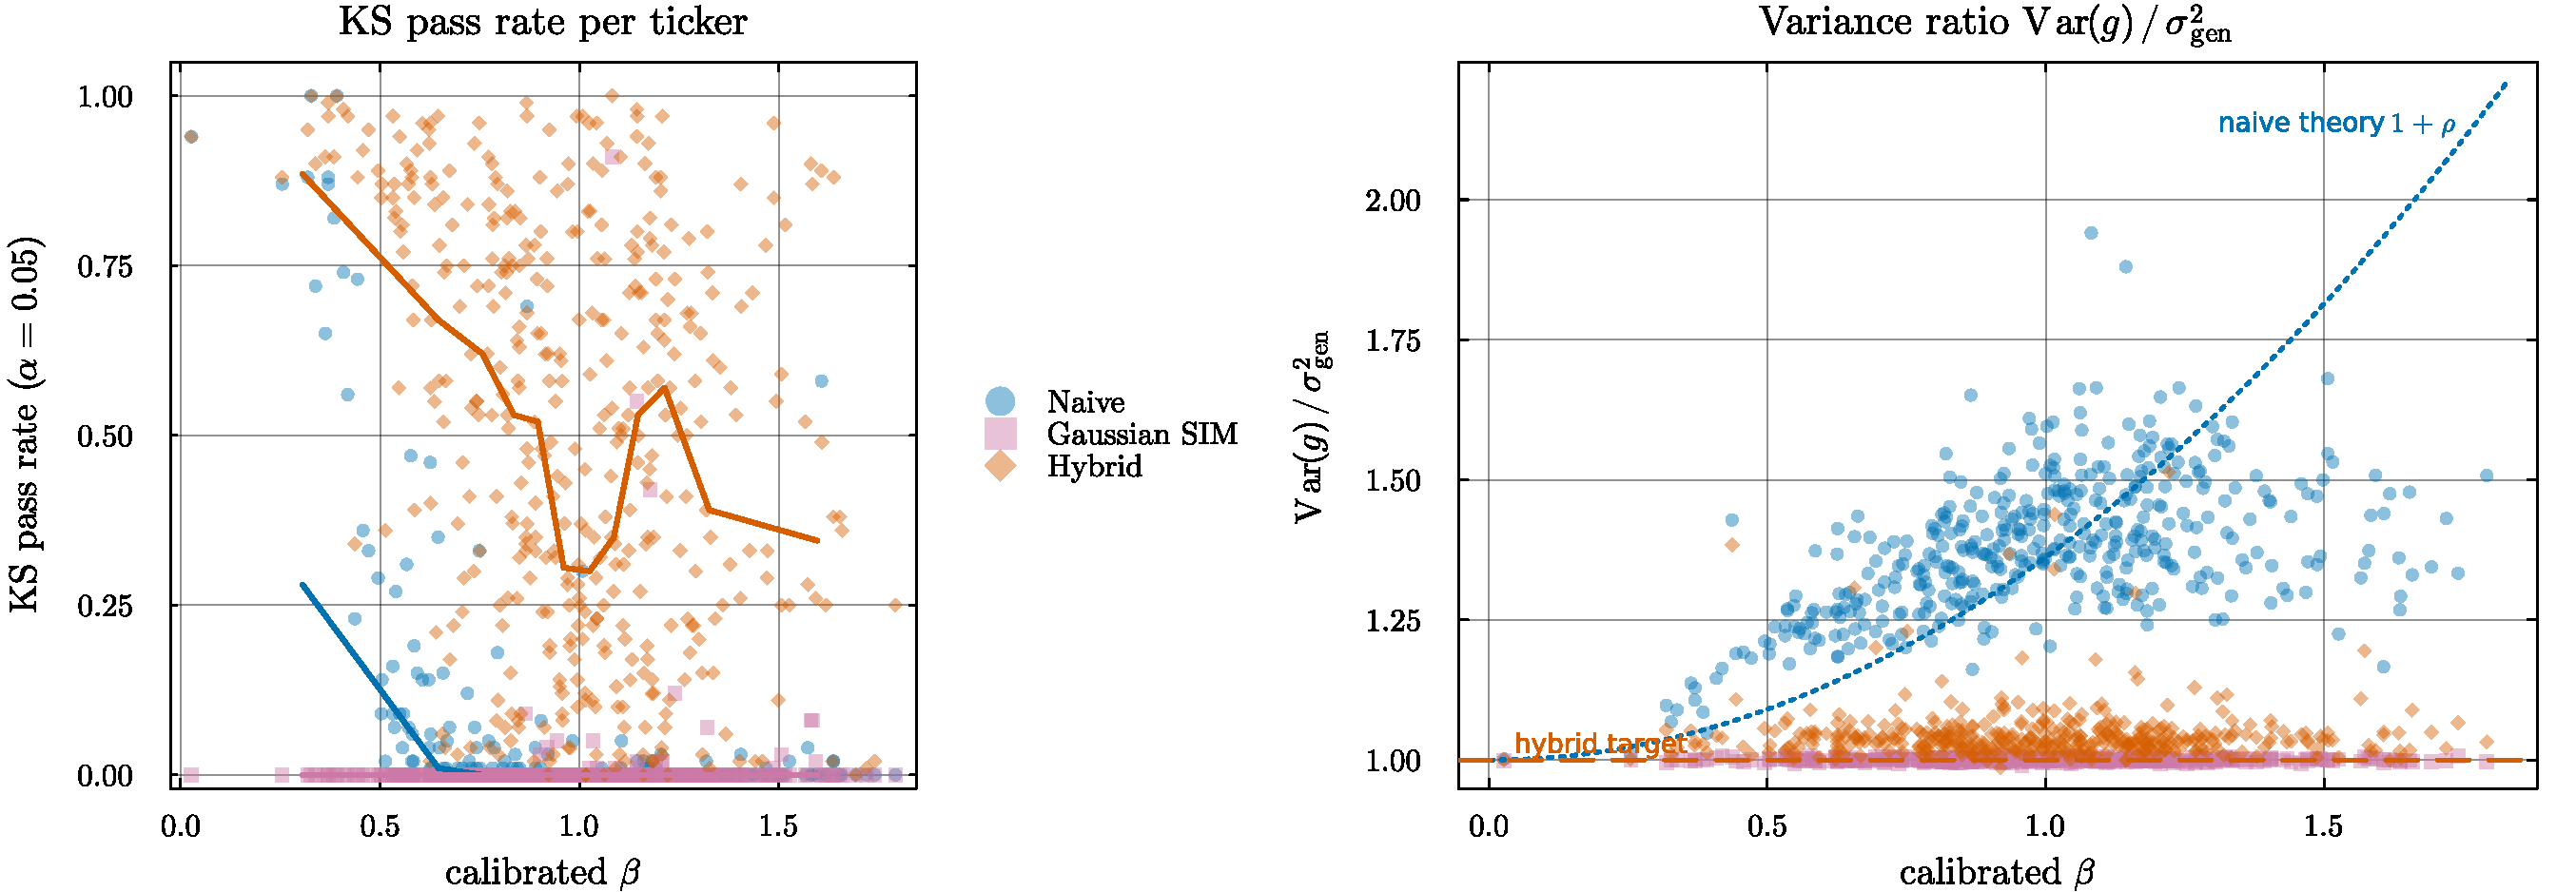
\includegraphics[width=\textwidth]{figs/fig1_preservation.pdf}
  \caption{\textbf{Marginal-distribution preservation and variance
    preservation vs calibrated $\beta$.}
    Each point is a per-ticker median over $100$ replications.
    \emph{Left:} Kolmogorov--Smirnov pass rate against the real marginal
    at $\alpha = 0.05$. The hybrid composer (orange) maintains a pass
    rate between $\sim 0.3$ and $\sim 0.9$ across the full $\beta$ range;
    the naive composer (blue) collapses past $\beta \approx 0.7$ as the
    market loading inflates the marginal variance; the Gaussian SIM
    baseline (purple) is pinned at zero throughout.
    \emph{Right:} variance ratio $\mathrm{Var}(g)/\sigma^2_{\mathrm{gen}}$.
    The dotted curve is the theoretical naive inflation $1 + \rho$
    evaluated at the universe-median $\sigma^2_{\mathrm{gen}}$; the naive
    scatter follows it. Hybrid and Gaussian SIM sit on the unit line by
    design.}
  \label{fig:preservation}
\end{figure}

% -----------------------------------------------------------------------
% Figure 2: Tails and kurtosis
% -----------------------------------------------------------------------
\begin{figure}[p]
  \centering
  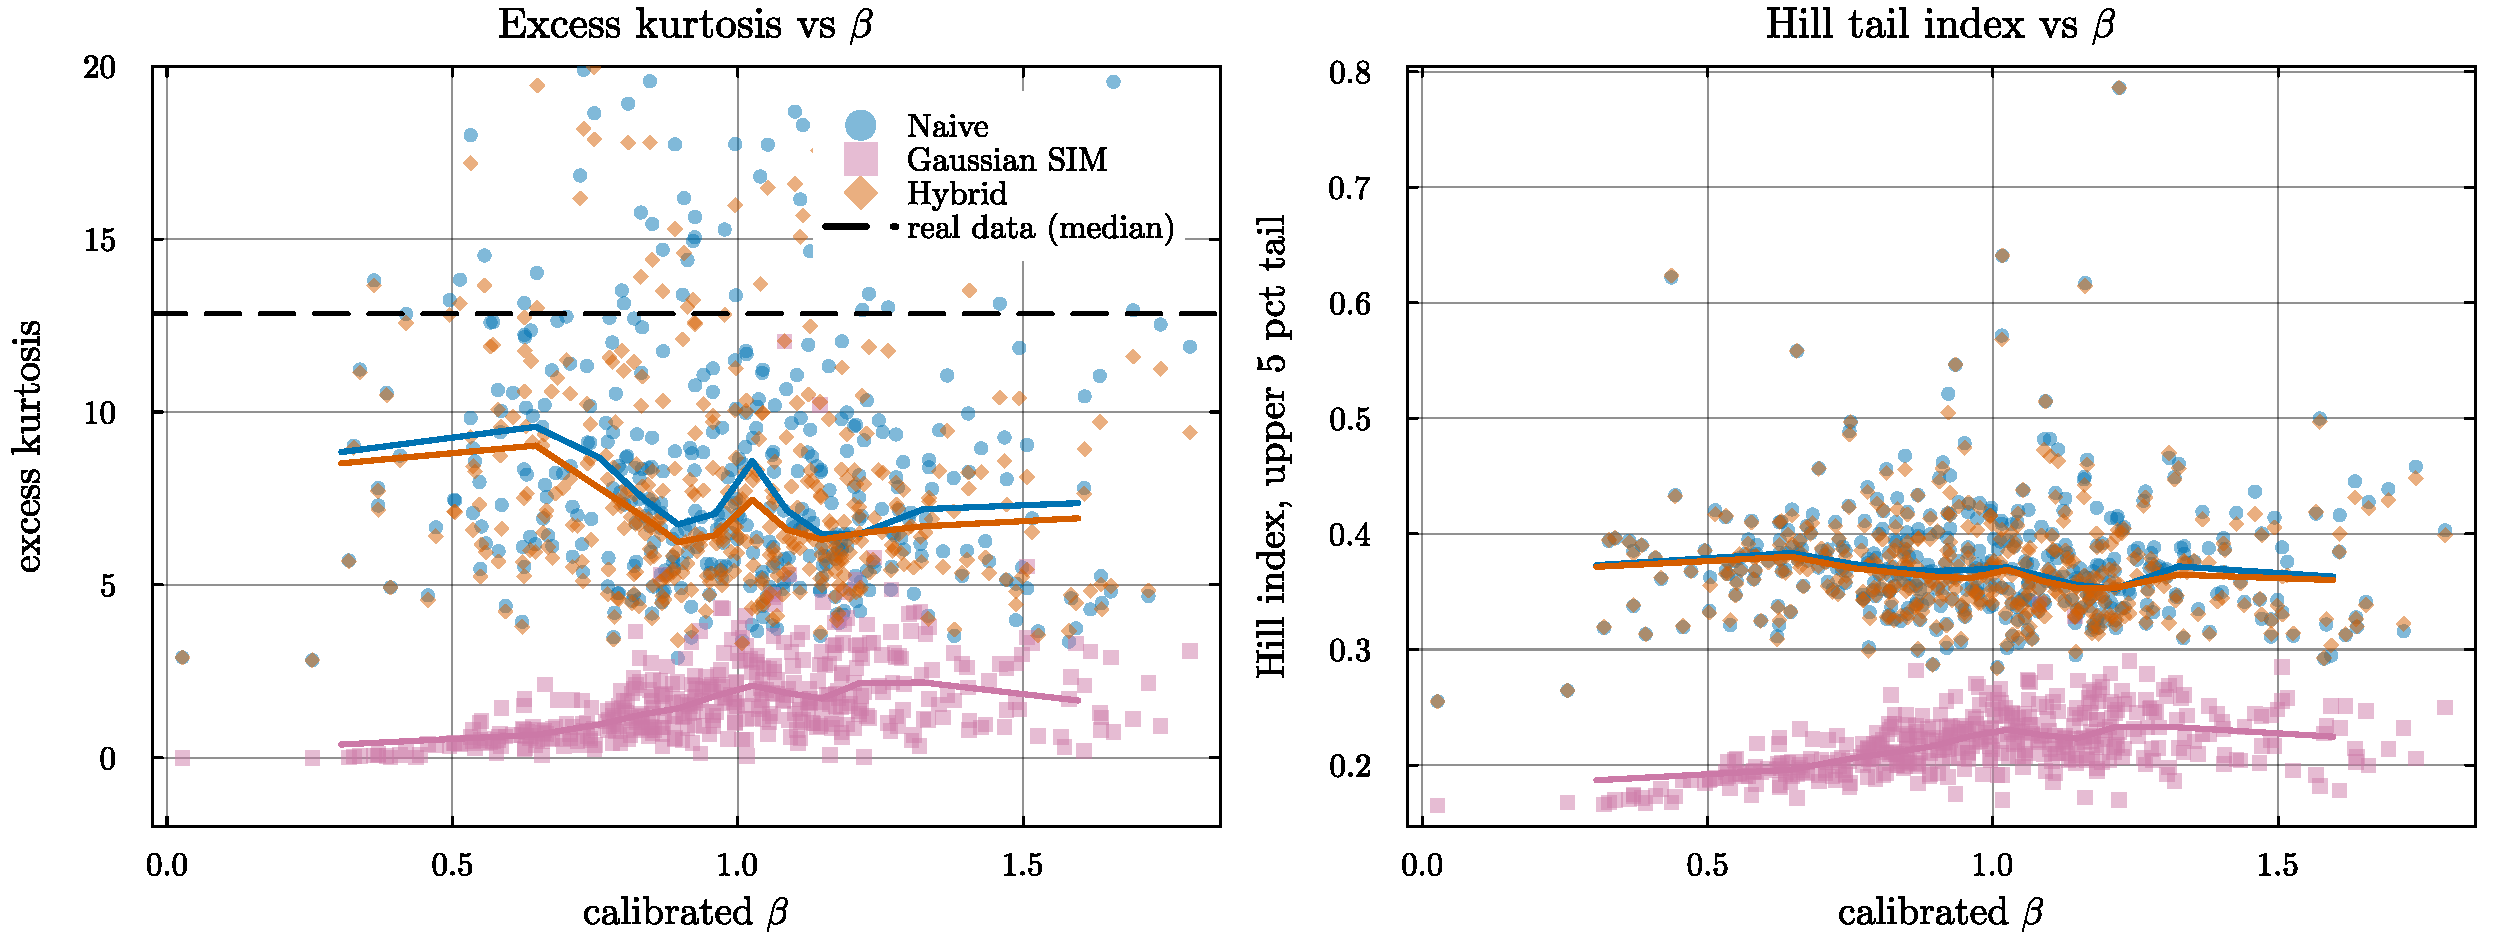
\includegraphics[width=\textwidth]{figs/fig2_tails.pdf}
  \caption{\textbf{Heavy-tail preservation: excess kurtosis and Hill
    tail index vs calibrated $\beta$.}
    Each point is a per-ticker median over $100$ replications.
    \emph{Left:} excess kurtosis, $y$-axis clipped to $[-2, 20]$ for
    readability. The dashed line marks the median real-data excess
    kurtosis across the universe ($\kappa_{\real} \approx 13$); the
    hybrid and naive composers (orange and blue) track the generator's
    kurtosis, while Gaussian SIM collapses to $\kappa \approx 1$.
    \emph{Right:} Hill tail-index estimator on the upper $5\%$ of
    $|g|$. The hybrid and naive medians sit near $0.37$ throughout the
    $\beta$ range; Gaussian SIM drops to $\sim 0.22$, indicating the
    shift toward a thinner-tailed distribution. The hybrid's median
    sitting below $\kappa_{\real}$ reflects the JumpHMM marginal's own
    kurtosis rather than a composition-rule distortion; the panel's
    point is that hybrid tracks naive (inheriting generator tails)
    while Gaussian SIM does not.}
  \label{fig:tails}
\end{figure}

% -----------------------------------------------------------------------
% Figure 3: Branch map in (beta, R^2) space
% -----------------------------------------------------------------------
\begin{figure}[p]
  \centering
  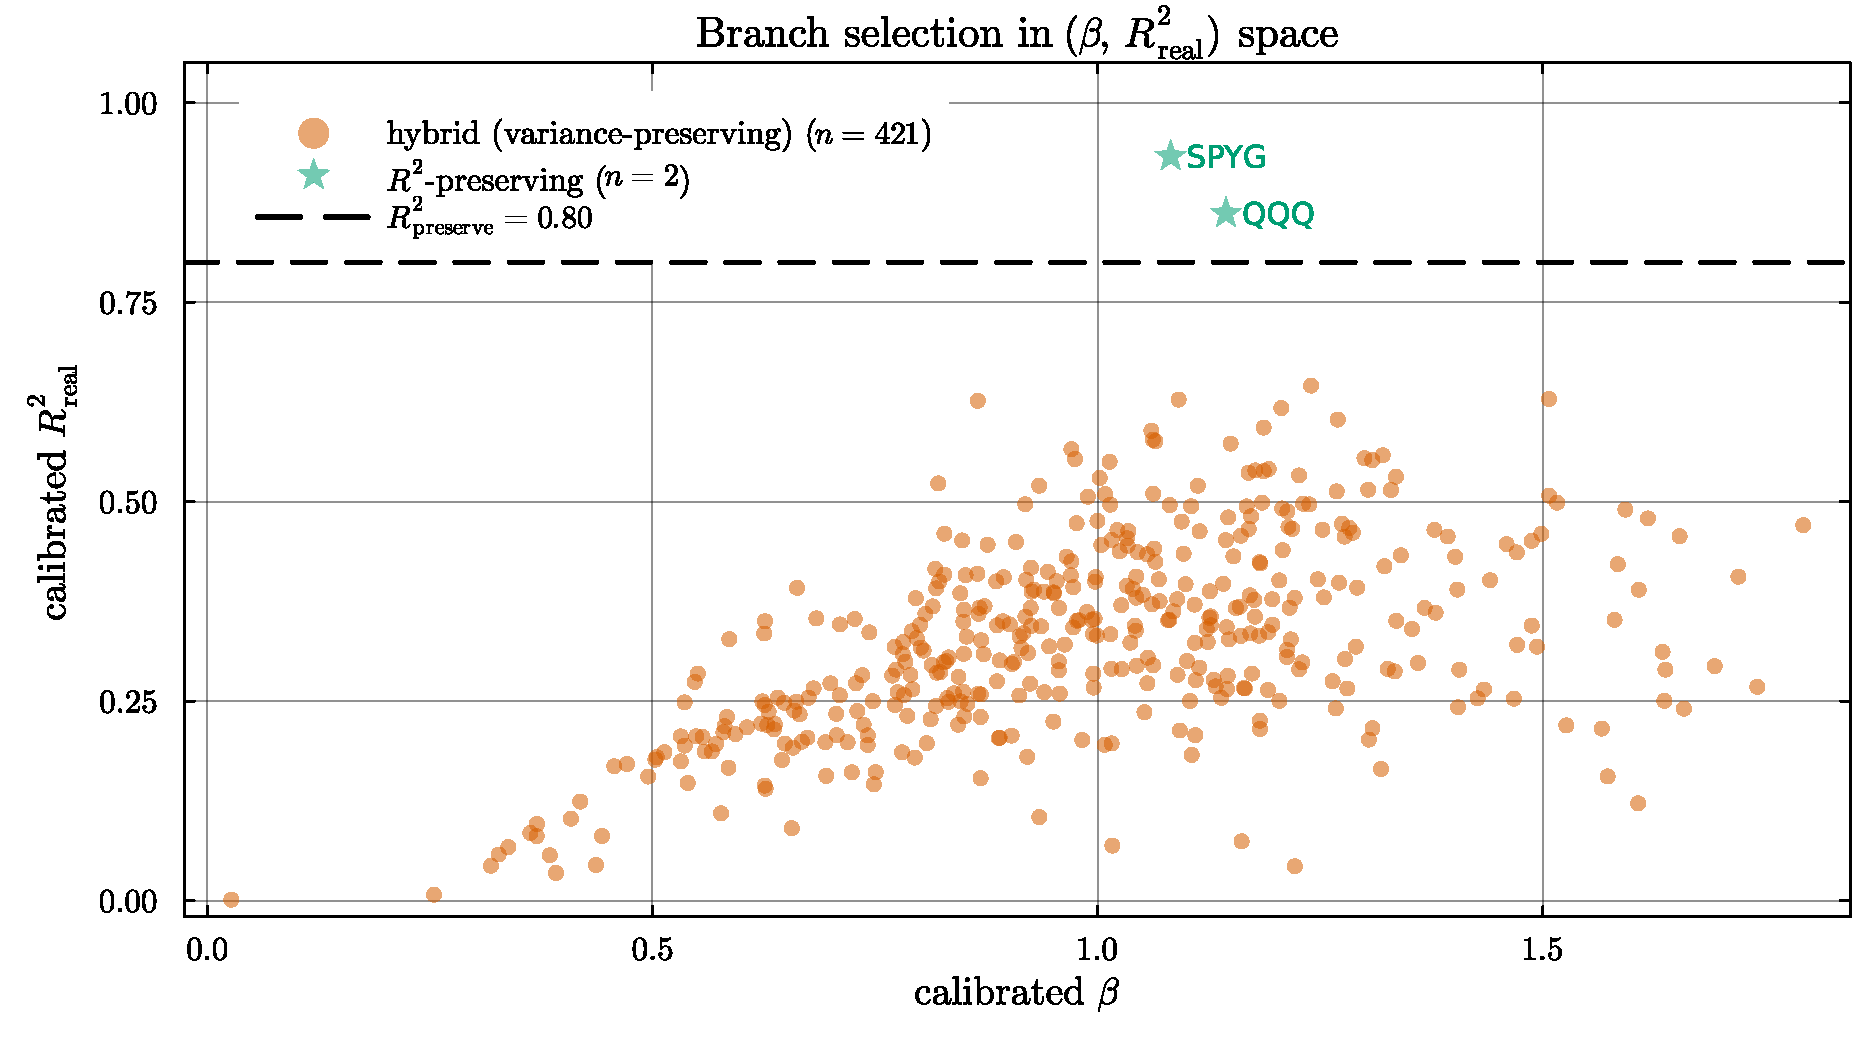
\includegraphics[width=0.85\textwidth]{figs/fig3_branch_map.pdf}
  \caption{\textbf{Construction-flag assignment in calibrated
    $(\beta, R^2_{\real})$ space.}
    The $R^2_{\mathrm{preserve}} = 0.80$ threshold (dashed line) separates
    tracker assets from genuine single stocks. In this universe, only
    QQQ and SPYG exceed the threshold, and both are assigned to the
    \texttt{r2-preserve} branch. The remaining $421$ tickers populate the
    \texttt{hybrid} (variance-preserving) branch; the
    \texttt{hybrid-clipped} branch is unused because the market loading
    ratio $\rho_i = \beta_i^2 \sigma_m^2 / \sigma_{\gen,i}^2$ stays
    below $0.90$ for every ticker.}
  \label{fig:branch_map}
\end{figure}

% --- SI Appendix (no supplemental material at this stage) ---

\end{document}
